% mnras_template.tex
%
% LaTeX template for creating an MNRAS paper
%
% v3.0 released 14 May 2015
% (version numbers match those of mnras.cls)
%
% Copyright (C) Royal Astronomical Society 2015
% Authors:
% Keith T. Smith (Royal Astronomical Society)

% Change log
%
% v3.0 May 2015
%    Renamed to match the new package name
%    Version number matches mnras.cls
%    A few minor tweaks to wording
% v1.0 September 2013
%    Beta testing only - never publicly released
%    First version: a simple (ish) template for creating an MNRAS paper

%%%%%%%%%%%%%%%%%%%%%%%%%%%%%%%%%%%%%%%%%%%%%%%%%%
% Basic setup. Most papers should leave these options alone.
\documentclass[a4paper,fleqn,usenatbib]{mnras}

% MNRAS is set in Times font. If you don't have this installed (most LaTeX
% installations will be fine) or prefer the old Computer Modern fonts, comment
% out the following line
%\usepackage{newtxtext,newtxmath}
\usepackage{import}
\usepackage{hyperref}

% Depending on your LaTeX fonts installation, you might get better results with one of these:
%\usepackage{mathptmx}
%\usepackage{txfonts}

% Use vector fonts, so it zooms properly in on-screen viewing software
% Don't change these lines unless you know what you are doing
\usepackage[T1]{fontenc}
\usepackage{ae,aecompl}

\usepackage{graphicx}	% Including figure files
\usepackage{amsmath}	% Advanced maths commands
\usepackage{amssymb}	% Extra maths symbols
\usepackage{pdflscape}	% Landscape pages
\usepackage[utf8]{inputenc}
\usepackage{multirow}
\usepackage{float} % here for H placement parameter

%%%%%%%%%%%%%%%%%%%%%%%%%%%%%%%%%%%%%%%%%%%%%%%%%%

%%%%% AUTHORS - PLACE YOUR OWN COMMANDS HERE %%%%%

% Please keep new commands to a minimum, and use \newcommand not \def to avoid
% overwriting existing commands. Example:
%\newcommand{\pcm}{\,cm$^{-2}$}	% per cm-squared

%%%%%%%%%%%%%%%%%%%%%%%%%%%%%%%%%%%%%%%%%%%%%%%%%%

%%%%%%%%%%%%%%%%%%% TITLE PAGE %%%%%%%%%%%%%%%%%%%

% Title of the paper, and the short title which is used in the headers.
% Keep the title short and informative.
\title[A reference transient dataset I: lightcurves]{A reference
  dataset for astronomical transient event recognition I: lightcurves
  and tests on classical machine learning algorithms}


% The list of authors, and the short list which is used in the headers.
% If you need two or more lines of authors, add an extra line using \newauthor
\author[M. Neira et al.]
{Mauricio Neira$^{1}$, Catalina G\'omez$^{2}$, Diego A. G\'omez $^{1}$,
Marcela Hern\'andez Hoyos$^{1}$,   
\newauthor
Jaime E. Forero-Romero$^{3}$,
Pablo Arbel\'aez$^{2}$
\\
% List of institutions
$^{1}$Systems and Computing Engineering Department, Universidad de los Andes, Cra. 1 No. 18A-10, Bogot\'a, Colombia\\
$^{3}$Departamento de Ingenier\'ia Biom\'edica, Universidad de los Andes, Cra. 1 No. 18A-10, Bogot\'a, Colombia\\
$^{2}$Departamento de F\'isica, Universidad de los Andes, Cra. 1 No. 18A-10, Bogot\'a, Colombia
}

% These dates will be filled out by the publisher
\date{Accepted XXX. Received YYY; in original form ZZZ}

% Enter the current year, for the copyright statements etc.
\pubyear{2019}

% Don't change these lines
\begin{document}
\label{firstpage}
\pagerange{\pageref{firstpage}--\pageref{lastpage}}
\maketitle

% Abstract of the paper
\begin{abstract}

We introduce ATRANCCA (Annotated TRANsient Catalina CAtalog) an
annotated dataset of $4869$ transient and $16940$ non-transient
object light-curves built from the Catalina Real Time Transient
Survey.
We provide access to this dataset as a plain text file to facilitate
standarized quantitative comparison of astronomical transient event
recognition algorithms. 
The classes included in the dataset are: supernovae, cataclismic
variables, active galactic nuclei, high proper motion stars, blazars
and flares.
As an example on how to use the dataset we experiment with multiple
data pre-processing methods, feature selection techniques and classic
machine learning algorithms (Support Vector Machines, Random Forests
and Neural Networks).   
We assess quantitative performance in two classification tasks:
binary (transient/non-transient) and eight-class classification.   
The best performing algorithm is a Random Forest Classifier for both
classification experiments.  
The next release of ATRANCCA will include images and benchmarks with
deep learning models. 
All our code and data is available to the community at
\url{https://github.com/MachineLearningUniandes/ATRANCCA}.
\end{abstract}

% Select between one and six entries from the list of approved keywords.
% Don't make up new ones.
\begin{keywords}
methods: data analysis, statistical
%keyword1 -- keyword2 -- keyword3
\end{keywords}

%%%%%%%%%%%%%%%%%%%%%%%%%%%%%%%%%%%%%%%%%%%%%%%%%%

%%%%%%%%%%%%%%%%% BODY OF PAPER %%%%%%%%%%%%%%%%%%

\section{Introduction}

The study and detection of astronomical variable sources is expected
to occur on unprecedented scales with the new generation of
forthcoming multi-epoch and multi-band (synoptic) astronomical
surveys. 
For instance, projects like the Large Synoptic Survey Telescope
(LSST)  \citep{0805.2366,1512.07914} are expected to generate
exuberant daily data-streams near to 20 petabytes every night.   

One of the main challenges that these datasets want to address is
Real-Time Transient classification, i.e. flagging astrophysically
relevant events whose luminosity varies in short duration relative in
the timescale of the Universe, from minutes to several years.  
Transients include phenomena such as supernovae, novae, neutron
stars, blazars, pulsars, cataclysmic variable stars (CV), gamma ray
bursts (GRB) and active galaxy nuclei (AGN). 
The time-domain dependency of these objects is one of the reasons why
they are hard to classify: their data is usually heterogeneous,
unbalanced, sparse, unevenly sampled and with missing information. 
This has motived the use of Machine Learning (ML) algorithms to recognize
and classify transient events. 


There have been successful attempts to implement these algorithms
using images as an input.
For instance, data from the SkyMapper Supernova and Transient
Survey and the High cadence Transient Survey (HiTS) have been used as
inputs to automatic detection algorithms \citep{1708.08947,1701.00458}.
Convolutional Neural Networks (CNN) have also achieved
high accuracy in this binary classification task.
Other studies have shown that artifacts can be detected using
features extracted from raw images. 
\cite{1601.06320} achieved reliable
classification by transforming transient data from the OGLE-IV
data-reduction pipeline and training it with machine learning
algorithms such as Artificial Neural Networks, Support Vector
Machines, Random Forests, Naive Bayes, K-Nearest Neighbors and Linear
Discriminant Analysis.  
Similarly, \cite{1501.05470} used images from Pan-STARS1 Medium Deep
Surveys, and \cite{1407.4118} processed single-epoch multi-band images
from the SDSS supernova survey for the same purpose.  


A complementary approach uses the light curves computed from the
images to perform the classification task.
For instance \cite{1601.03931} used classical machine learning
algorithms such as Random Forest, MultiLayer Perceptron and K-Nearest Neighbours
light curves to classify transients from the Catalina Real Time
Transient Survey; \cite{1603.00882} used the same approach to find
where supernovas from the Supernova Photometric Classification
Challenge.

A crucial element in the developmet of any ML algorithm is the
compilation of the training dataset. 
In astronomy this task has been facilitated by the publication of
large databases from different observational projects. 
However, the publications that make use of these datasets still make
extensive use of the internal know-how of the scientific
collaboration. 
It is still difficult for another scientists to rebuild a training
dataset and perform comparisons with published results.

To address this issue we compile and publish in easy-to-access files a
dataset that can be used to train and test different ML algorithms for
transient detection.
We use public data from the Catalina Real-Time Transient Survey
(CRTS) \citep{1111.2566}, an astronomical survey searching transient
and highly variable objects as base for the dataset.
In this paper we present light-curve data, in a future publication we
will present an imaging dataset. 

In Section \ref{sec:data} we present the CRTS and the steps we follow
to build the dataset.
In Section \ref{sec:repository} we describe its main features together
with the repository structure gathering the files and some Python code  
to explore it.
In Section \ref{sec:ml_tests} we show how this dataset can be used to
perform some tests using some classical ML tests follow a similar
approach as \cite{1601.03931}.  
We finalize in Section \ref{sec:conclusions} with a summary of main
features of our dataset and the results of our ML tests.

\section{The lightcurve dataset} \label{section_data}

We use public data from the Catalina Real-Time Transient Survey
(CRTS) \citep{2009ApJ...696..870D}, an astronomical survey searching transient
and highly variable objects.   
It covered 33000 squared degrees of sky and took data since 2007.
Three telescopes were used: Mt. Lemmon Survey (MLS), Catalina Sky
Survey (CSS), and Siding Spring Survey (SSS). So far, CRTS has
discovered more than $15000$ transient events.
We use light curves as measured with the CSS telescope of the CRTS, which is
an f/1.8 Schmidt telescope located in the Santa Catalina Mountains, north of Tucson,
Arizona and is equipped with a 111-megapixel  detector, and covered
4000 square degrees per night, with a limiting magnitude of 19.5 in
the V band.  
Details about the observations, data reduction and transient
detection can be found in \cite{2009ApJ...696..870D}
The public CRTS data base (\url{http://crts.caltech.edu/}) reports the
source magnitudes and its corresponding uncertainty. 


The CRTS dataset already provides a classification. 
The most numerous classes are: supernovae (SN),
cataclysmic variable stars (CV), blazars, flares, asteroids, active
galactic nuclei (AGN), and high-proper-motion stars (HPM). 
Though most objects in the transient object catalogue belong to a single class,
there is some uncertainty in the categorization of some of
them. 
In this case, an interrogation sign is used when a class is not clear
e.g. SN? or sometimes multiple possible classes are found for a single
event e.g. SN/CV.
Table \ref{Top-Transient-Classes} summarizes the number of objects in
each class. 

The lightcurves were directly provided from the CRTS project.
To compile the non-transient dataset we retrieve sources in the
dataset from the CRTS online catalogue by sampling light curves of
objects within a 0.006  degree radius from CRTS detected transients,
and removing known transient light curves from that set. 
Our dataset includes all lightcurves with at least one observation. 

% Number of transients per transient class
\begin{table}
\centering
\begin{tabular}{c|c}
    \hline
    Class &  Object Count \\
    \hline
SN & 1723 \\
CV & 988 \\
HPM & 640 \\
AGN & 446 \\
SN? & 319 \\
Blazar & 243 \\
Unknown & 228 \\
Flare & 219 \\
AGN? & 138 \\
CV? & 77 \\
    \hline
\end{tabular}
\caption{Top 10 transient classes, with their respective number of
  light-curves.} 
\label{table:top_clases}
\end{table}




\section{Repository Description} \label{section_code}

The repository that contains the light-curves and some code to process
the data can be found in
\url{https://github.com/MachineLearningUniandes/ATRANCCATA}. 

The repository has three main folders

\begin{itemize}

\item \texttt{data/lightcurves}: 
Contains three text files in CSV format
the transient light curves (\texttt{transient\_lightcurves.csv}),
the labels for the transients (\texttt{transient\_labels.csv}) and
the light curves for non-transient objects
(\texttt{nontransient\_lightcurves.csv}). 
The first two files can be linked by unique transient IDs and
provided in the CRTS database. 
\item \texttt{nb-explore}: includes a jupyter notebook
  (\texttt{explore\_light\_curves.ipynb}) with examples on how to read
  and plot transient and non-transient light curves (Figure
  \ref{fig:examples_transient} and Figure
  \ref{fig:examples_non_transient}), extract the statistic in Table
  \ref{table:top_classes} and prepare the summary statistics in Figure
  \ref{fig:cumulative}. 
\item{\texttt{ML}}: Contains the data sets and notebooks to perform the ML
  tests. It is divided into three different directories:
\begin{itemize}
\item \texttt{notebooks}. Contains all the code for the ML tests. 
  There are three numbered jupyter notebooks summarizing our
  experimental framework.  
  The documentation is included into each notebook.
  There are various \texttt{.py} files with the required python
  routines. 
\item \texttt{features}:  resulting features of pre-processing the
light curves for both transients and non-transients. 
\item \texttt{inputs} data-set split into training/test for the
  different machine learning classification tasks. 
  Data is split into different meta-parameters:
  classification task, number of features, minimum number of
  observations, and balanced/unbalanced data. 
  Each one of the input files contains a numpy tuple with the
  structure: \textit{(train features, train labels, test features,
    test labels)}  
\item \texttt{results}. Products of the ML test. 
  One result type is named dataframes, which contains a pandas
  dataframe for each task. 
  Each dataframe contains the testing and
  training results, including scores and confusion matrices.  
  On the other hand, the results sub-folder contains the feature
  importance list figures presented in this document.  
\end{itemize}
\end{itemize}


\begin{figure*}
	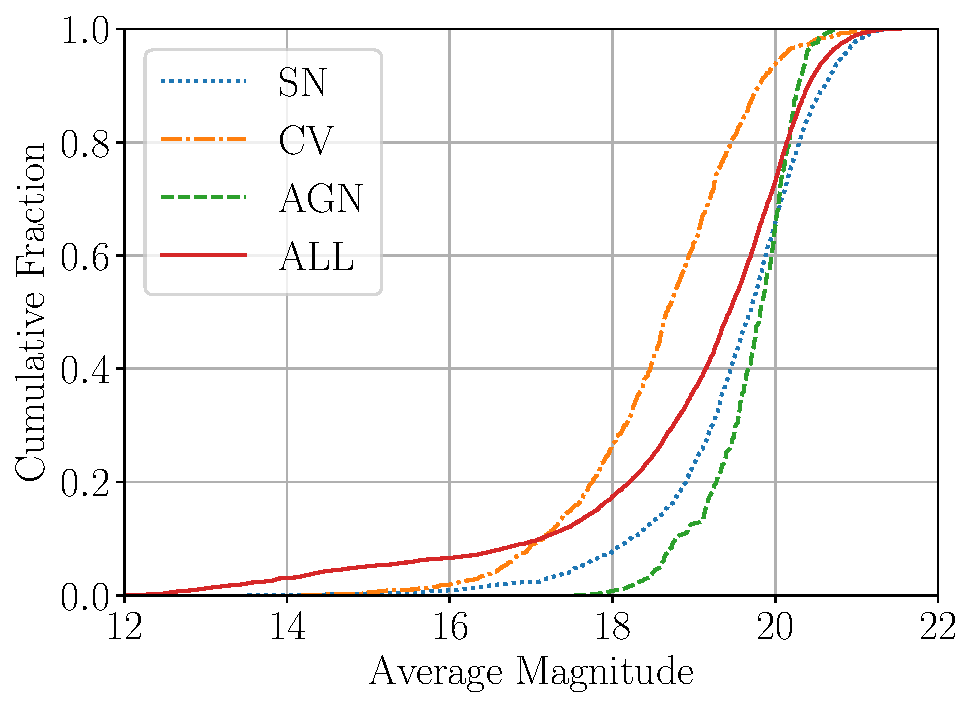
\includegraphics[width=0.45\textwidth]{cumulative_magnitude.pdf}
  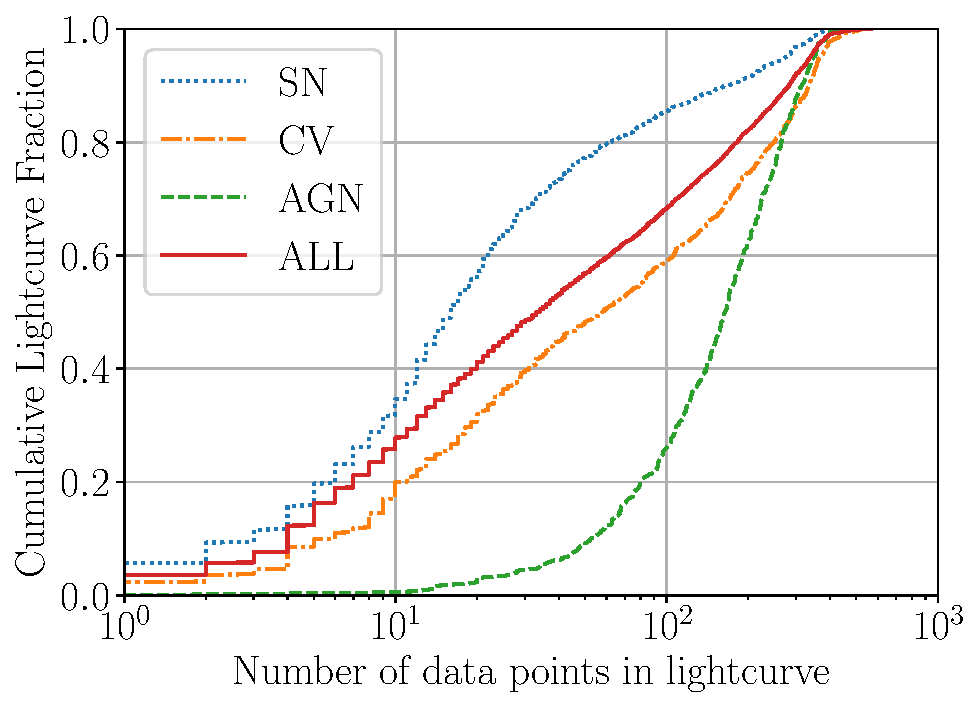
\includegraphics[width=0.45\textwidth]{cumulative_classes.pdf}
  \caption{Cumulative number of light curves (expressed as a fraction)
    as a function of average magnitude (left) and number of data
    points in the light curve (right).
    This includes information for the three most representative
    classes (SN, CV, AGN) and the whole database (ALL).}
  \label{fig:cumulative}
\end{figure*} 



\begin{figure*}
  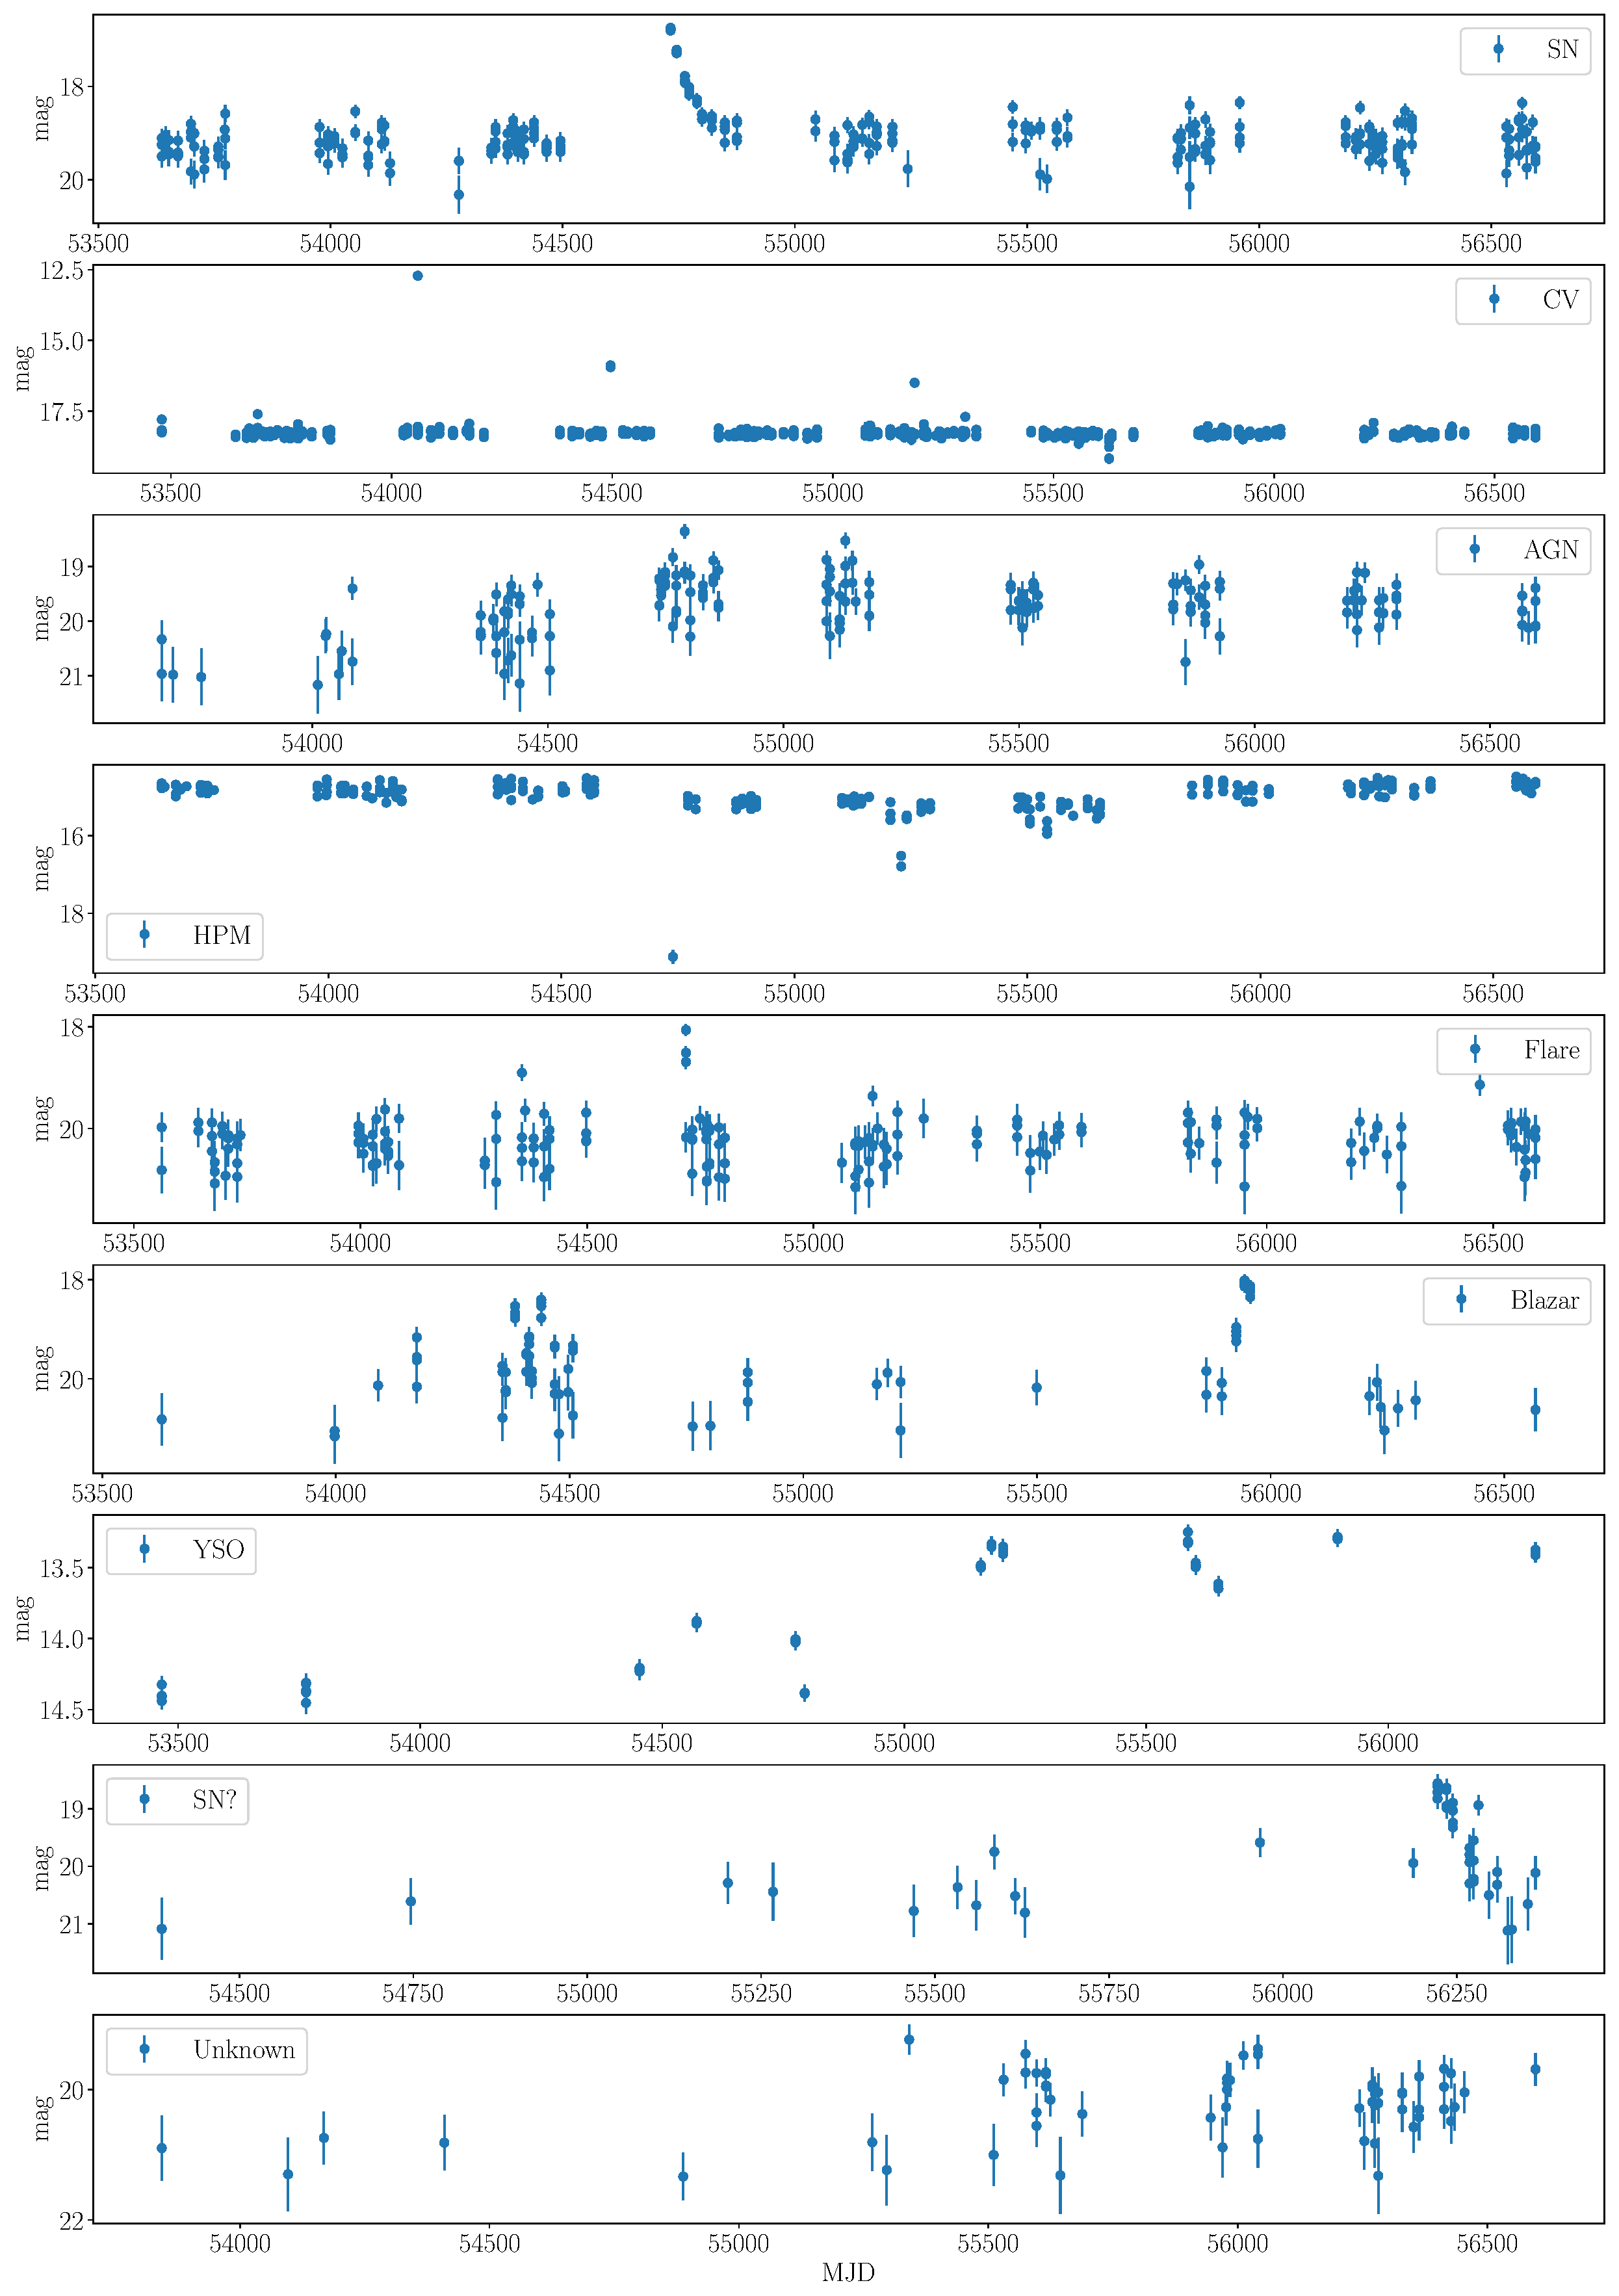
\includegraphics[width=0.8\textwidth]{examples_transient.pdf}
  \caption{Randomly selected lightcurves for the most represented classes as
    compiled in the database we present in this paper.}  
  \label{fig:examples_transient}
\end{figure*} 


\begin{figure*}
  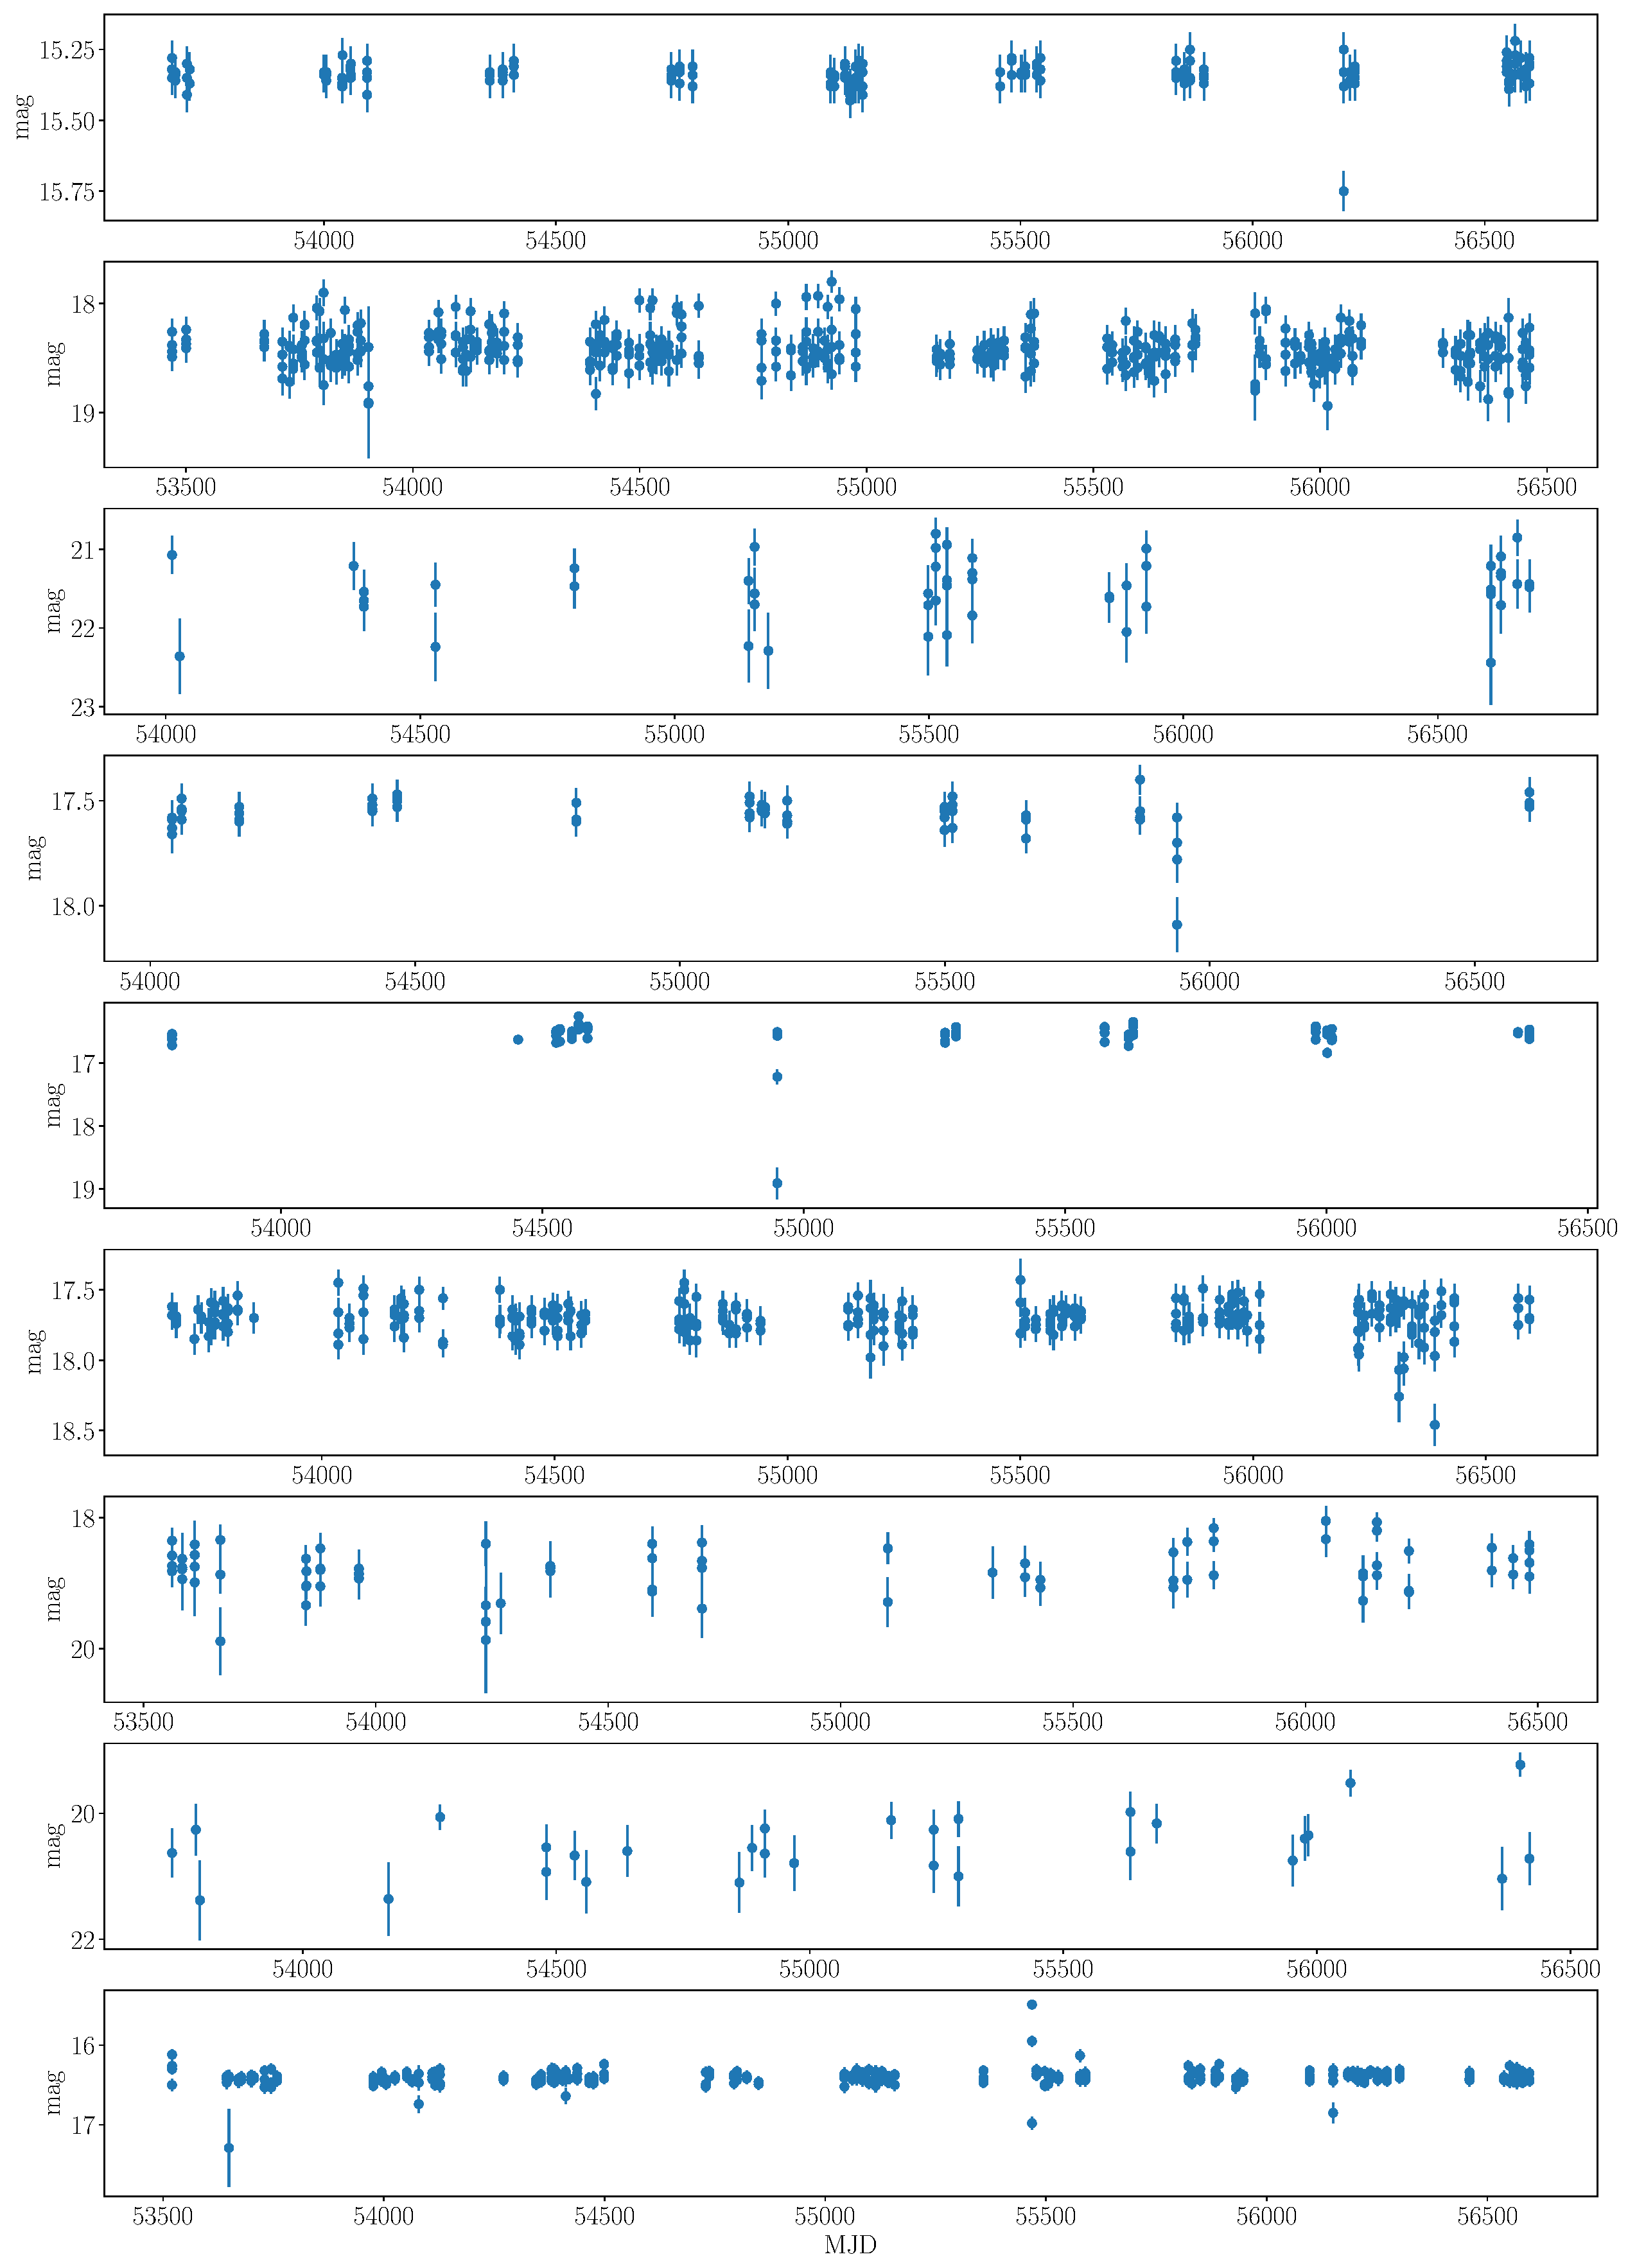
\includegraphics[width=0.8\textwidth]{examples_nontransient.pdf}
  \caption{Randomly selected lightcurves for non-transient sources.}
  \label{fig:examples_non_transient}
\end{figure*} 




%The tables \ref{Transient-Observation-Count} and
%\ref{Non-Transient-Observation-Count} summarize the 
%number of light curves of  transient and non-transient sources, respectively, that
%contain at least 5 observations. 
%Each of these tables present the mean, standard deviation, percentiles
%(25, 50 and 75) and maximum number of observations per light curve
%found in each dataset. 

% Number of transients per transient class
%\begin{table}
%\centering
%\begin{tabular}{c|c}
%    \hline
%    Count & 4269 \\
%    \hline
%    Mean & 102.810 \\
%    Std & 113.786 \\
%    Min & 5 \\
%    25\% & 14 \\
%    50\% & 48 \\
%    75\% & 166 \\
%    Max & 564 \\
%    \hline
%\end{tabular}
%\caption{Transient's data-set observation count per object.}
%\label{Transient-Observation-Count}
%\end{table}

% Number of transients per transient class
%\begin{table}
%\centering
%\begin{tabular}{c|c}
%    \hline
%    Count & 15193 \\
%    \hline
%    Mean & 118.37 \\
%    Std & 116.51 \\
%    Min & 5 \\
%    25\% & 26 \\
%    50\% & 72 \\
%    75\% & 185 \\
%    Max & 537 \\
%    \hline
%\end{tabular}
%\caption{Non-Transient's data-set observation count per object.}
%\label{Non-Transient-Observation-Count}
%\end{table}



\section{Classical Machine Learning Tests} \label{section_method}

As an example on how the dataset can be used, we apply classical
machine learning algorithms to perform different classification tasks.


\subsection{Data Preprocessing}
We do not feed directly the anotated lightcurves to the ML algorithms.
There is preprocessing stage that follows six steps.

\subsubsection{Data Filtering} \label{subsection_filtering}

We discard light curves with few observations as they may not contain
enough information to be classified correctly
Our nominal cut is 10 observations per light curve.


\subsubsection{Oversampling Transient Light Curves} \label{subsection_oversampling}

The number of light curves per class is unbalanced. 
In order to have the same amount elements for each class we implement an
oversampling step by artificially generating multiple mock light curves,
each based on an observed one. 

We generate a mock light curve from the observed light curve and 
then sample the observed magnitude from a Gaussian distribution
centered on the observational apparent magnitude with the magnitude's
error as the standard deviation. 


\subsubsection{Feature Extraction} \label{subsection_extraction}

Light curves are sampled at irregular time intervals and have
different numbers of data points.
Thus, it is challenging to directly use the time-series data for
classification with traditional methods.
We circumvent this problem by extracting a set of features for each
light curve.
These features are scalars derive from statistical and model-specific
fitting techniques. 
The first features (moment-based, magnitude-based and
percentile-based) were formally introduced in 
\cite{1101.1959}, and have been used in other studies \citep{1603.00882,1601.03931}.  
We extend that list to include another set (polynomial fitting-based features. 
These groups are:

\begin{enumerate}
    
\item Moment-based features, which use the magnitude for each light curve.
  \begin{itemize}
  \item \underline{Beyond1std} (\textit{beyond1std}): 
    Percentage of observations which are over or under one standard
    deviation from the weighted average. Each weight is calculated as
    the inverse of the corresponding observation's photometric error. 
        \item \underline{Kurtosis} (\textit{kurtosis}): 
        The fourth moment of the data distribution. Used to measure
        the heaviness or lightness in the tails of the statistical
        data. 
        \item \underline{Skewness} (\textit{skew}): 
        A measurement of the level of asymmetry from the normal
        distribution in a data distribution. Negative skewness is the
        property of a more pronounced left tail, while positive
        skewness is a characteristic that implies a more pronounced
        right tail. 
        \item \underline{Small Kurtosis} (\textit{sk}):
        Small sample kurtosis.
        \item \underline{Standard deviation} (\textit{std}):
        The standard deviation of the magnitudes.
        \item \underline{Stetson J} (\textit{stetson\textunderscore j}):
        The Welch-Stetson J variability index
        \cite{1996PASP..108..851S}. A robust standard deviation. 
        \item \underline{Stetson K} (\textit{stetson\textunderscore k}): 
        The Welch-Stetson K variability index
        \cite{1996PASP..108..851S}. A robust kurtosis measure. 
    \end{itemize}
    
    \item Magnitude-based features, which rely on the magnitude for each source.
    \begin{itemize}
    \item \underline{Amplitude} (\textit{amp}): 
      The difference between the maximum and minimum magnitudes.
    \item \underline{Max Slope} (\textit{max\textunderscore slope}): 
      Maximum absolute slope between two consecutive observations.
    \item \underline{Median Absolute Deviation} (\textit{mad}): 
      The median of the difference between magnitudes and the median
      magnitude. 
    \item \underline{Median Buffer Range Percentage} (\textit{mbrp}): 
      The percentage of points within 10\% of the median magnitude.
    \item \underline{Pair Slope Trend} (\textit{pst}): 
      Percentage of all pairs of consecutive magnitude measurements that have positive slope.
    \item \underline{Pair Slope Trend 30} (\textit{pst\textunderscore last30}): 
      Percentage of the last 30 pairs of consecutive magnitudes that have a positive slope, minus percentage of the last 30 pairs of consecutive magnitudes with a negative slope.
    \end{itemize}


  \item Percentile-based features, which use the sorted flux distribution for
    each source. The flux is computed as $F = 10^{0.4 \mathrm{mag}}$. 
    We define $F_{n,m}$ as the difference between the $m$-th and $n$-the flux
    percentiles. 
    \begin{itemize}
    \item \underline{Percent Amplitude} (\textit{p \textunderscore amp}): 
      Largest percentage difference between the absolute maximum magnitude and the median.
    \item \underline{Percent Difference Flux Percentile} (\textit{pdfp}): 
      Ratio between $F_{5,95}$ and the median flux.
    \item \underline{Flux Percentile Ratio Mid20} (\textit{fpr20}): 
      Ratio $F_{40,60} / F_{5,95}$
    \item \underline{Flux Percentile Ratio Mid35} (\textit{fpr35}):
        Ratio $F_{32.5,67.5} / F_{5,95}$
      \item \underline{Flux Percentile Ratio Mid50} (\textit{fpr50}): 
        Ratio $F_{25,75} / F_{5,95}$
      \item \underline{Flux Percentile Ratio Mid65} (\textit{fpr65}): 
        Ratio $F_{17.5,82.5} / F_{5,95}$
      \item \underline{Flux Percentile Ratio Mid80} (\textit{fpr80}): 
        Ratio $F_{10,90} / F_{5,95}$
    \end{itemize}
    
  \item Polynomial Fitting-based features, which are the coefficients of
    multi-level terms in a polynomial curve fitting. This is new set
    of features proposed in this paper. 
    \begin{itemize}
        \item \underline{Poly1 T1}: Linear term coeff. in monomial curve fitting.
        \item \underline{Poly2 T1}: Linear term coeff. in quadratic curve fitting.
        \item \underline{Poly2 T2}: Quadratic term coeff. in quadratic curve fitting.
        \item \underline{Poly3 T1}: Linear term coeff. in cubic curve fitting.
        \item \underline{Poly3 T2}: Quadratic term coeff. in cubic curve fitting.
        \item \underline{Poly3 T3}: Cubic term coeff. in cubic curve fitting.
        \item \underline{Poly4 T1}: Linear term coeff. in quartic curve fitting.
        \item \underline{Poly4 T2}: Quadratic term coeff. in quartic curve fitting.
        \item \underline{Poly4 T3}: Cubic term coeff. in quartic curve fitting.
        \item \underline{Poly4 T4}: Quartic term coeff. in quartic curve fitting.
    \end{itemize}    
\end{enumerate}


\subsubsection{Feature Scaling} \label{subsection_scaling}

We re-scale the magnitudes to have zero mean  and unit variance. 


\subsection{Classification Tasks} \label{subsection_classification}

We study two classification tasks.

\subsubsection{ Binary Classification}
We use a balanced number of events from both classes in order 
to investigate the capability of distinguishing between Transients
and Non-Transients.

\subsubsection{8-Class Classification}

We consider the unbalanced number of objects across classes to 
perform a classification into the following categories:
AGN, Blazar, CV, Flare, HPM, Other, Non-Transient and Supernovae.   


\subsection{ML algorithms}


We conduct experiments with three widely used families of supervised classification 
algorithms: Neural Networks (NNs), Random Forests (RFs) and Support
Vector Machines (SVMs). 

These algorithms are popular in published studies and are efficient 
for low dimensional feature datasets as is our case. 
We use sklearn \citep{1201.0490} Python's implementation of these algorithms.
Details on the inner workings of these machine learning models can be
found in \cite{9780387848570}.  

The set of hyperparameter space explored for each algorithm is the
following. 

For Neural Networks:
\begin{itemize}
    \item Learning Rate: Either constant vs adaptive.
    \item Hidden Layer Sizes: Single Layer with $100$ nodes vs Two layers with
    $100$ nodes each.
    \item L2 Penalty ($\alpha$): 
      $10^{-1}$, $10^{-2}$, $10^{-3}$ , $10^{-4}$.
    \item Activation Function: Logistic vs Relu.
\end{itemize}

For Random Forest:
\begin{itemize}
    \item Number of Estimators: $200$ or $700$.
    \item Number of features Considered: Square Root or the Logarithm 
    base 2 of the total number of features.
\end{itemize}

For Support Vector Machines:
\begin{itemize}
    \item Kernel: Radial Basis Function (RBF).
    \item Kernel Coefficient ($\gamma$):  
      $10^{-1}$, $10^{-2}$, $10^{-3}$ , $10^{-4}$, $10^{-5}$
    \item Error Penalty (\textit{C}): 1 vs 10 vs 100 vs 1000. 
\end{itemize}


\subsection{Validation} \label{subsection_importances}

We split the input light curves in a training and test datasets. 
The test dataset contains only original light curves, without any
oversampling. 
We use 2-fold cross-validation during training as evaluation
protocol. 
Moreover, we use grid search during training to test multiple
hyper-parameter configurations for each one  of the possible
algorithms. 
We use the F1-Score to assess the performance of a given model and 
we evaluate each task on the held-out test dataset.


\begin{figure*}
	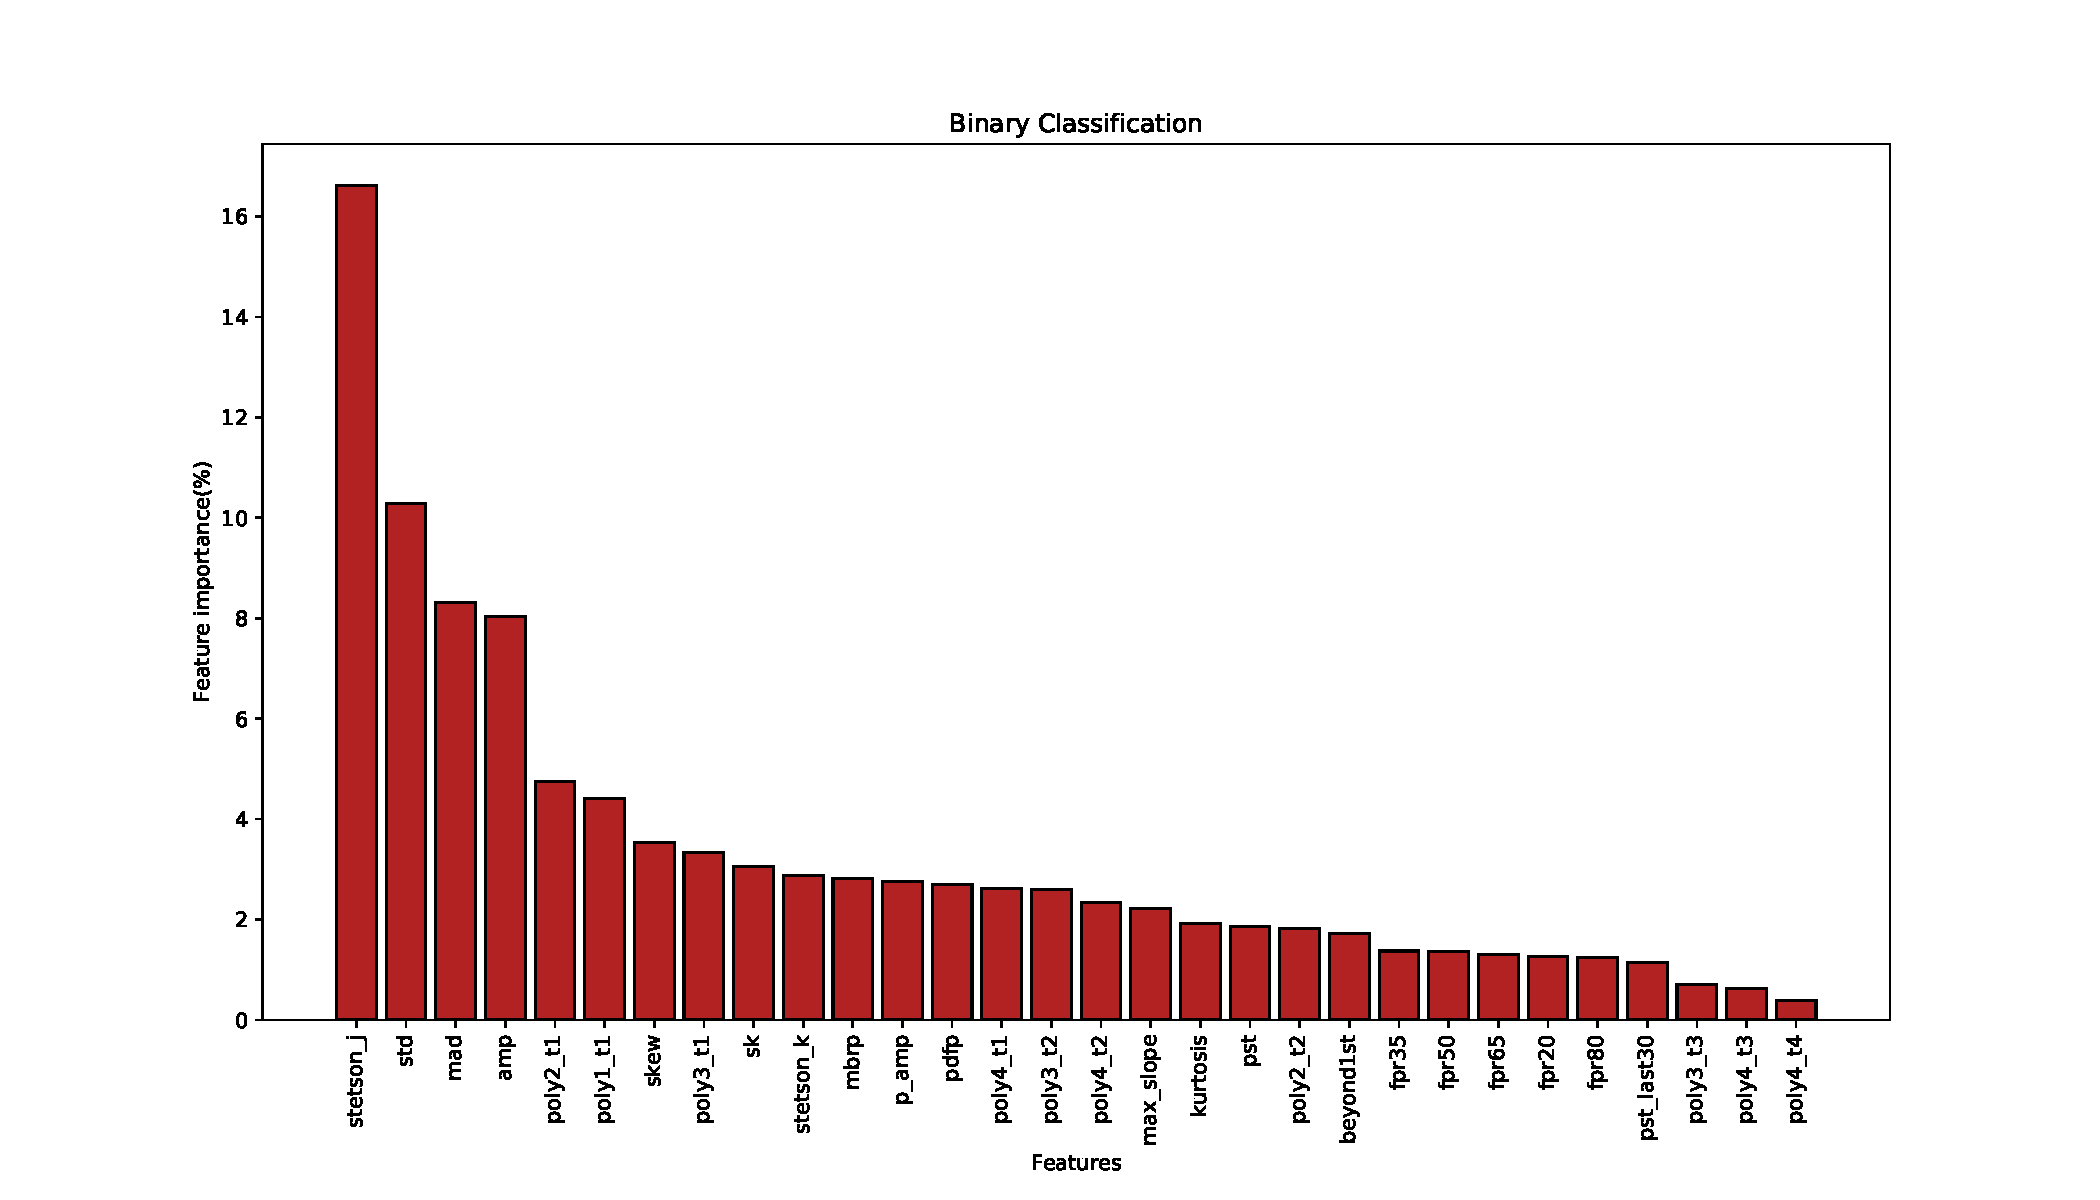
\includegraphics[width=\textwidth]{binFeatImportance.pdf}
    \caption{Feature importance rank  for the best Random Forest
      classifier for the Binary classification task. 
      Feature importance is represented with percentages.} 
    \label{Importances-Binary}
\end{figure*} 

\begin{figure*}
	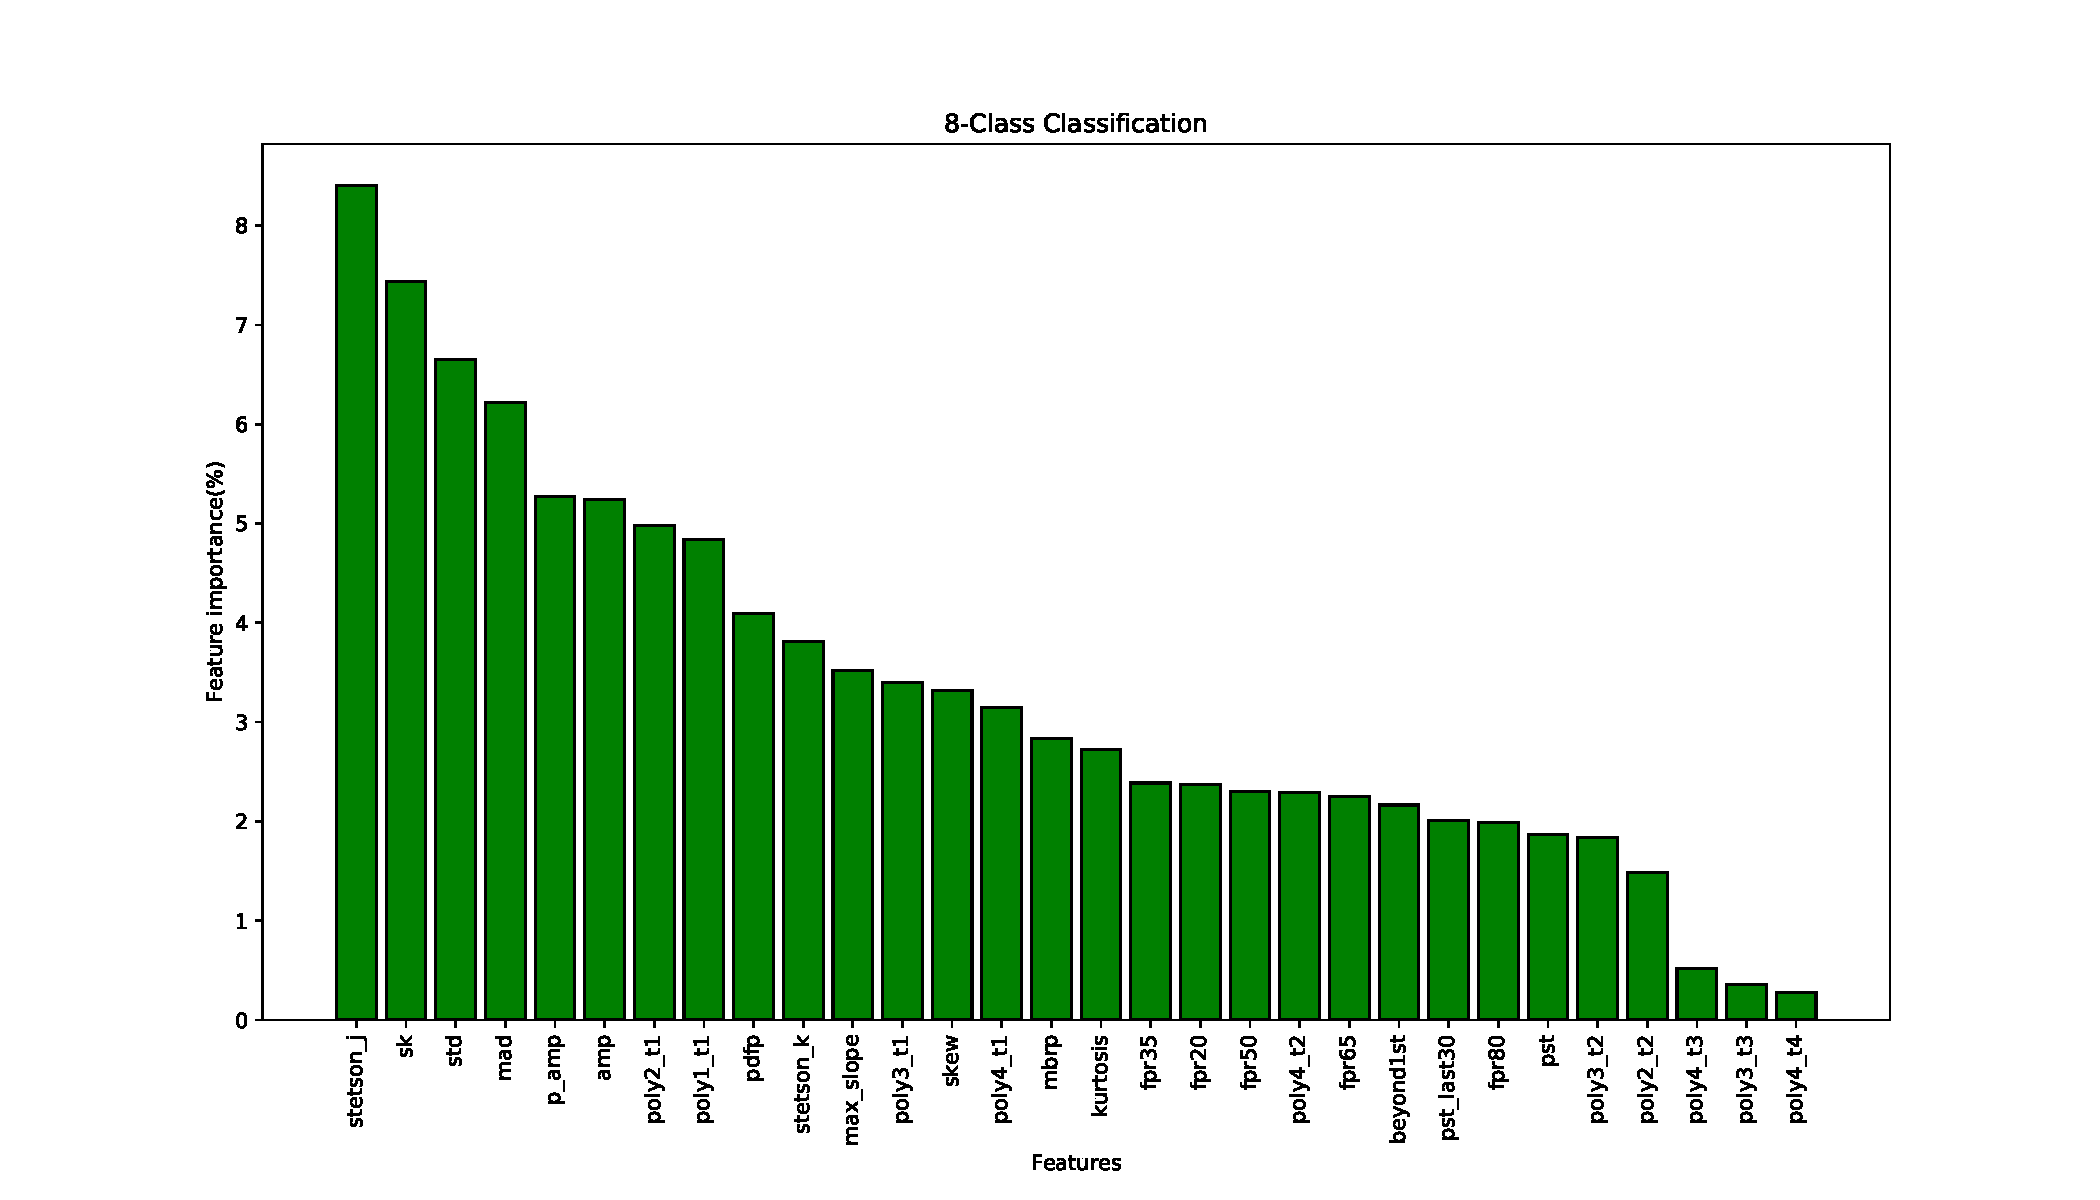
\includegraphics[width=\textwidth]{8classFeatImportance.pdf}
    \caption{Feature importance rank for the best Random Forest
      classifier for the best 8-Class classification task. Feature
      importance is represented with percentages.} 
    \label{Importances-8-Class}
\end{figure*}

\subsection{Results}

%%%%%%  BINARY  %%%%%%
\subsubsection{Binary Classification} 
\label{Results-Binary} 


The best algorithm in this task is RFs with a maximum F1-score of
87.69\%.   
SVMs are the second best-performing model with the F1-score of 85.36\%. 
Changing the number of features does not affect significantly the score.
NNs are ranked third, although their scores are very similar to those of SVMs. 
The highest achieved score for NNs is 85.03\%.


Table \ref{Confusion-Binary} shows the confusion matrix of the best
performing algorithm and Table \ref{Overall-Scores-Binary} summarizes
the scores.
These results imply that non-transients are better classified overall.  


Figure \ref{Importances-Binary} displays the most important features
for the RFs classifier.
The top five inputs for classification are stetson\textunderscore j,
std, mad, poly1\textunderscore t1 and poly2\textunderscore t1.  
The former achieved the highest importance with over 21\%, compared to
the following with values in the range 6\% - 8\%. 


\begin{table}
\centering
\begin{tabular}{|r|c|c|c|c|}
\hline
\multicolumn{1}{|l|}{} & Precision & Recall & f1-Score & Support \\ \hline \hline
Non-Transient          & 94.13     & 94.13      & 94.13      & 3798   \\ \hline
Transient              & 79.10     & 79.10      & 79.10      & 1067    \\ \hline
\end{tabular}
\caption{Precision, Recall and f1-score for the Binary Classification Task with Regular inputs.}
\label{Overall-Scores-Binary}
\end{table}

\begin{table}
\centering
\begin{tabular}{|r|c|c|}
\hline
\multicolumn{1}{|l|}{} & non-transient    & transient   \\ \hline \hline
non-transient                & 3575       & 223    \\ \hline
transient                    & 223       & 844   \\ \hline
\end{tabular}
\caption{Confusion Matrix for the best performing model in the Binary task.}
\label{Confusion-Binary}
\end{table}



%%%%%%  EIGHT-CLASS  %%%%%%
\subsubsection{Eight-Class Classification}


RFs are the best classifier. 
The best f1-score is 66.05\%. 
NNs are the second best. 
Its highest f1-score is 60.19\%, while SVMs are the worst-performing
model only achieving a maximum f1-score of 57.30\%.
Table \ref{Classifier-Scores-8-Class-10} summarizes the results. 


Table \ref{Confusion-8-Class} presents the confusion matrix for the RF.
The two classes with highest recall are HPM and Non-Transient, with a
recall of 86.36\% and 84.13\%, respectively. 
The worst performing classes are Blazar, Flare and Other, with recall
values in the range 36\% - 40\%. 
SN is the class with which most other class instances are
incorrectly classified. 
Moreover, Flares have about 50\% of the test samples classified as
Non-Transients, AGNs have about 20\% of their 
samples classified as Other, and Blazars and Other had most of  its
samples classified as AGN. 
Additionally, most incorrectly classified AGNs ($\sim$20.5\%) are
identified as Other and most Blazar instances are
incorrectly categorized as either SN or AGN. 


Figure \ref{Importances-8-Class} displays the feature importance ranking.
This list ranks first stetson\textunderscore j with an 8\% importance,
followed by amp, sk, std, mad, with values around 6\%. 
The lowest raking features are the five high level polynomial: poly4\textunderscore
t1,  poly4\textunderscore t2, poly3\textunderscore t3,
poly4\textunderscore t3 and poly4\textunderscore t4. 


\begin{table}
\centering
\begin{tabular}{|r|c|c|c|c|}
\hline
\multicolumn{1}{|l|}{} & Precision & Recall & f1-Score & Support \\ \hline \hline
SN            &   48.82 &   51.39  &  50.07  &  323 \\ \hline
CV            &   66.96 &   70.69  &  68.77  &  215 \\ \hline
AGN           &   48.14 &   85.84  &  61.69  &  106 \\ \hline
HPM           &   25.19 &   86.84  &  39.05  &   76 \\ \hline
Blazar        &   46.77 &   49.15  &  47.93  &   59 \\ \hline
Flare         &    7.00 &   41.17  &  11.96  &   51 \\ \hline
Other         &   31.11 &   44.01  &  36.46  &  234 \\ \hline
Non-transient &   96.06 &   79.69  &  87.12  & 3798 \\ \hline
avg/total     &   46.25 &   63.59  &  50.38  & 4862 \\ \hline
\end{tabular}
\caption{Precision, Recall and f1-score for the 8-Class Classification Task with Regular inputs.}
\label{Overall-Scores-8-Class-Regular}
\end{table}

\begin{table*}
\centering
\begin{tabular}{|r|c|c|c|c|c|c|c|c|}
\hline
\multicolumn{1}{|l|}{} & SN    & CV    & AGN   & HPM   & Blazar   & Flare   & Other   & Non-Transient  \\ \hline \hline
SN            & 166  &  25  &  0  &  0  &  7   &  5  &  40 &   97 \\ \hline
CV            &  17  & 152  &  0  &  1  &  5   &  3  &  12 &   37 \\ \hline
AGN           &   1  &   2  & 91  &  0  & 10   &  1  &  35 &   49 \\ \hline
HPM           &   5  &   0  &  0  & 66  &  0   &  0  &   5 &  186 \\ \hline
Blazar        &   8  &  13  &  4  &  0  & 29   &  0  &   6 &    2 \\ \hline
Flare         &  16  &   5  &  0  &  0  &  3   & 21  &   4 &  251 \\ \hline
Other         &  53  &  12  &  7  &  1  &  3   &  3  & 103 &  149 \\ \hline
Non-Transient &  57  &   6  &  4  &  8  &  2   & 18  &  29 & 3027 \\ \hline
\end{tabular}
\caption{Confusion Matrix for the best performing model in the 8-Class task.}
\label{Confusion-8-Class}
\end{table*}



\section{Conclusions}

The scope of forthcoming of large astronomical synoptic surveys 
motivates the development and exploration of automatized ways to
detect transient sources. 
In turn this prompts the compilation of publicly available databases
to train and test new algorithms. 
In this paper we presented the results of such compilation based on data
from the Catalina Real-Time Transient Suvey (CRTS).
The data-set compiles  $4869$ transient and $16940$ non-transient
light-curves. 
The dataset is publicly available at
\url{https://github.com/MachineLearningUniandes/ATRANCCA}.   

We illustrated how to use this database by extracting 
characteristic features to use them as inputs to train three different
machine learning algorithms (Random Forests, Neural Networks and
Support Vector Machines) for classification tasks.
The features extracted from light curves were either statistical
descriptors of the observations, or polynomial curve fitting
coefficients applied to the light curves.   
Overall the best classifier for all tasks was the Random Forest.
In this model the most important feature was always stetson$\_$j.

In a second paper we will present another reference dataset for
astronomical transient event recognition based on images of the
CATALINA survey. 
The corresponding tests will use  state-of-the art deep learning
techniques for transient classification. 

\section*{Acknowledgements}

We thank Andrew Drake for sharing with us the CRTS Transient dataset
used in this project.  
We thank Juan Pablo Reyes, Dominique Fouchez for helping with the
research.  
We acknowledge funding from Universidad de los Andes in the call for
project finalization.
We also thank contributors and collaborators of the SciKit-Learn,
Jupiter Notebooks and Pandas' Python libraries.  

CRTS and CSDR2 are supported by the U.S.~National Science 
Foundation under grant NSF grants AST-1313422, AST-1413600, and 
AST-1518308.  The CSS survey is funded by the National Aeronautics
and Space Administration under Grant No. NNG05GF22G issued through
the Science Mission Directorate Near-Earth Objects Observations Program.

\bibliographystyle{mnras}
\bibliography{bibliography}

\end{document}

